\chapter{The Effect of Data Gap Filling on Sensible Heat Flux Calculations}
\bigskip
\begin{spacing}{1}
\begin{center}
\textit{This chapter was written as a final project for CE 506: Theory and Measurement of Turbulent Fluxes, April 28th, 2016. Figures are in their original format.}\\
\end{center}
\bigskip
\noindent \textbf{Abstract}\\
\noindent The flux dataset collected during the Norwegian Young Sea Ice Cruise (N-ICE) project had a number of problems. The most restricting problem being the number of data gaps throughout the 30-minute pre-processed data files. In some cases, the amount of missing data made the file unable to be processed. In order to fix this, the data was filled by taking the section of data before it (or after, in the case that the missing data was too close to the start of the dataset) and replicating it for the time period with no recorded data. To ensure that this method of data filling was acceptable, data from Barrow, Alaska was used to compare the post-processed data of a complete dataset with the post-processed results from the same dataset after (artificially added) gaps had been filled. Analysis of both the difference in sensible heat fluxes and the turbulent spectra from before and after the data filling were examined and determined the filling method appropriate for the type of gaps in the N-ICE data. 
\end{spacing}
\doublespacing

\section{Introduction}
The Norwegian Young Sea Ice Cruise (N-ICE) project occurred from February 2015 to June 2015 (5 months). The primary objective of the project was to understand the ice dynamics and energy flux in the Arctic associated with young sea ice. Measurements were taken above newly formed sea ice while the R/V Lance research ship, used as a base for the researchers and a powerhouse for the equipment, flowed with the ice \citep{granskog:2016}. The eddy flux data collected during N-ICE is currently still in the processing phase. Any sections of missing data must first be repaired to ensure the complete dataset can be processed without the removal of any files. The main goal of this paper is to determine if the filling method used was an appropriate method by examining if it disturbed patterns or drastically changed heat flux values.

A large number of gaps exist in the N-ICE atmospheric turbulence data. These gaps could occur for a number of reasons, including rime ice accumulation on instruments, extreme cold temperatures \citep{cohen:2006}, issues with the power supply to the instruments, computer, or datalogger, and the packing up and moving of the instruments. The flux datasets from this experiment are in 30-minute files, often with small gaps of missing data within the file time period. It is important to patch these small data gaps, as too many can reduce the number of files that can be processed through the Licor processing software EddyPro \citep{epro, epro_man} 

Some data-filling methods include using the mean diurnal variation or using look-up tables. The mean diurnal variation method takes the mean of the half-hour before the gap in missing data and fills the gap with that mean. In the look-up table method, meteorological variations and other forcings can be taken into consideration \citep{falge:2001} For this dataset, however, a different approach was used. It did not seem appropriate to fill this minute with the mean of the previous half-hour because the gaps in data being filled were approximately around one minute in length. In addition, the half-hour before these gaps likely had a number of data gaps, too. The approach to gap-filling described in this paper is based on taking the values immediately before (or after) the data gap, and replacing the missing data values with them, essentially duplicating the previous minute.

This paper begins with a more detailed description of all data used. This is followed by an examination of the data-filling method used, including both a time-series analysis and a look at the spectra of the fluctuations. This paper will conclude with a description of future work to be done and a summary of the results presented here. 

\section{Methods}
The primary objective of this project is to determine a method to fill the dataset from N-ICE. From January 2015 to June 2015, a ship was frozen into newly forming sea ice in the Arctic ocean \citep{granskog:2016}. An array of instruments was installed onboard the ship, making measurements of temperature, wind speed, wind direction, fluctuations in water vapor, and carbon dioxide, which can be used to calculate heat fluxes. The dataset collected by these instruments is the focus of this project, with the goal of conducting the most accurate possible sensible and latent heat flux calculations using EddyPro. 

A major problem with the dataset was the existence of semi-regular data gaps throughout the collection period. These chunks of missing data appeared approximately every 5 minutes and lasted for about a minute. While these gaps were not present in every file, they could be found throughout the majority of the collection period. In addition to these semi-regular data gaps, irregular data gaps of varying duration also existed but occurred at a much lower rate. For the majority of the dataset, the spacing and duration of gaps were consistent.

There were much larger gaps in the data, too, where the instrument was likely taken down for the ship to be moved. Gaps lasting more than a 30-minute data file were regarded as breaks in data collection (instead of missing data) and no data filling was attempted for these time periods. The three largest data breaks were used to separate the data into three separate time periods, primarily for plotting purposes. These periods are 14 February 2015 through 18 February 2015, 9 March 2015 through 18 March 2015, and 24 April 2015 through 6 June 2015.  

As EddyPro reads the files and begins to process them, it checks for missing data. The threshold of missing data that is allowed can be changed, and for this project, the missing data allowance was set to 33 $\%$ missing data. This missing data allowance means that 30-minute input files that had less than 66 $\%$ data collection during that time period would not be used in the calculation of the fluxes. If a file was missing more than 33 $\%$ of the data due to missing gaps, the file was removed from processing. To ensure all collected data is used, every file must be made to contain less than 33 $\%$ data. 
 
 To create a complete dataset, these semi-regular and irregular (shorter than 30-minute) gaps had to be filled. The filling method selected for this project took the time period before the gap and inserted it into the time period of the gap for every measured variable. In other words, in each gap, the minute before the gap was repeated. If there was not enough data before the gap to use in the filling, the data from after the gap was used (as each 30-minute file was filled separately from one another, previous files were not used). It is important to note that the same time period was selected for each variable for each gap to fill the gap, conserving any correlations between fluxes in different variables that may exist.  

To ensure that this data-filling technique was accurately portraying the fluxes that might have been occurring, another dataset was used for comparison. Three sets of files collected in Barrow, Alaska from 2012 were used. While Barrow does not have the exact same conditions as the N-ICE project, it is in a similar climate and is a relatively close representation of the N-ICE conditions. The time periods of Barrow data were 2 April 2012 at 01:30 to 04:30, 24 May 2012 at 16:30 to 25 May 2012 at 14:30, and 9 June 2012 at 14:30 to 20:30. These files were of the same format as the N-ICE data, but contained no gaps.  The correct fluxes of this dataset could be calculated because of the completeness of the files. Regular gaps throughout the entire dataset are likely the worst-case scenario, as one-minute gaps every 5 minutes would not only remove small eddies occurring on less than a minute time scales could be removing patterns or eddies occurring on a 5-minute time scale. In addition, adding in the section of data before the gap could produce an artificial correlation, showing eddies occurring that did not actually exist. Because of this it was decided that regular gaps would be removed from the Barrow dataset for quality checking. 

\section{Results and Discussion}
\subsection{Barrow, Alaska – Quality Checking of Filling Algorithm}
\subsubsection{Mean Departures from Original Sensible Heat Flux}

For the April section of Barrow data, both the filled data and the data with gaps matched the original data very closely when sensible heat flux was calculated. This is displayed in Figure \ref{fig:barrow_flux} A. Figure \ref{fig:barrow_flux} B shows the percent differences in the data with gaps and the filled data from the original data. This was done by using Eq. \ref{eq:withgaps} and \ref{eq:withoutgaps}, respectively. All percent differences are less than 1, indicating that the calculated sensible heat flux for both the data with the gaps in it and the data that has been filled is close to the sensible heat fluxes calculated by the complete dataset.

\begin{equation}\label{eq:withgaps}
\frac{Data_{with gaps} - Data_{original}}{Data_{original}} \times 100
\end{equation}

\begin{equation}\label{eq:withoutgaps}
\frac{Data_{gap filled} - Data_{original}}{Data_{original}} \times 100
\end{equation}

The magnitude of the mean difference is 0.0316 $Wm^{-2}$ between the original data and the data with the gaps inserted into it. The mean difference between the original and the filled data is 0.0698 $Wm^{-2}$. The sensible heat flux calculated using the data with gaps in it was closer to the original sensible heat fluxes than that calculated with the filled data. However, both are small differences, so for the April case, the filling algorithm can be said to have done well.  The percent differences further attest to both cases fitting the original dataset well, as the larger percent difference from the original is less than 40 $\%$. With sensible heat values as small as they are in this section, it seems reasonable.

In the May case, the three data runs also closely followed the same sensible heat flux pattern. This is shown in Figure \ref{fig:barrow_flux} C, and the differences in EddyPro calculated sensible heat flux for this month are shown in Figure \ref{fig:barrow_flux} D. During this month, the mean differences between the filled data and the data with artificial gaps versus the original dataset calculations were very similar. The data with gaps had a mean difference from the original data of 0.1387 $Wm^{-2}$, and the filled data had a mean difference from the original of 0.1389 $Wm{-2}$. The files with the gaps inserted into them did a slightly better job than the filled data. All sensible heat fluxes were less than 10 $\%$ different from the calculated sensible heat fluxes from the full dataset. These percentages are much smaller than those seen with the April dataset as the sensible heat flux values are higher. For example, a change of the same magnitude in May would yield a lower percentage as the overall values are higher. This section contained the most points of the three Barrow datasets, with 28 data points, and shows that the filled data matches the original well. 


 \begin{figure}[h]
    \centering
        \vspace{-30pt}
    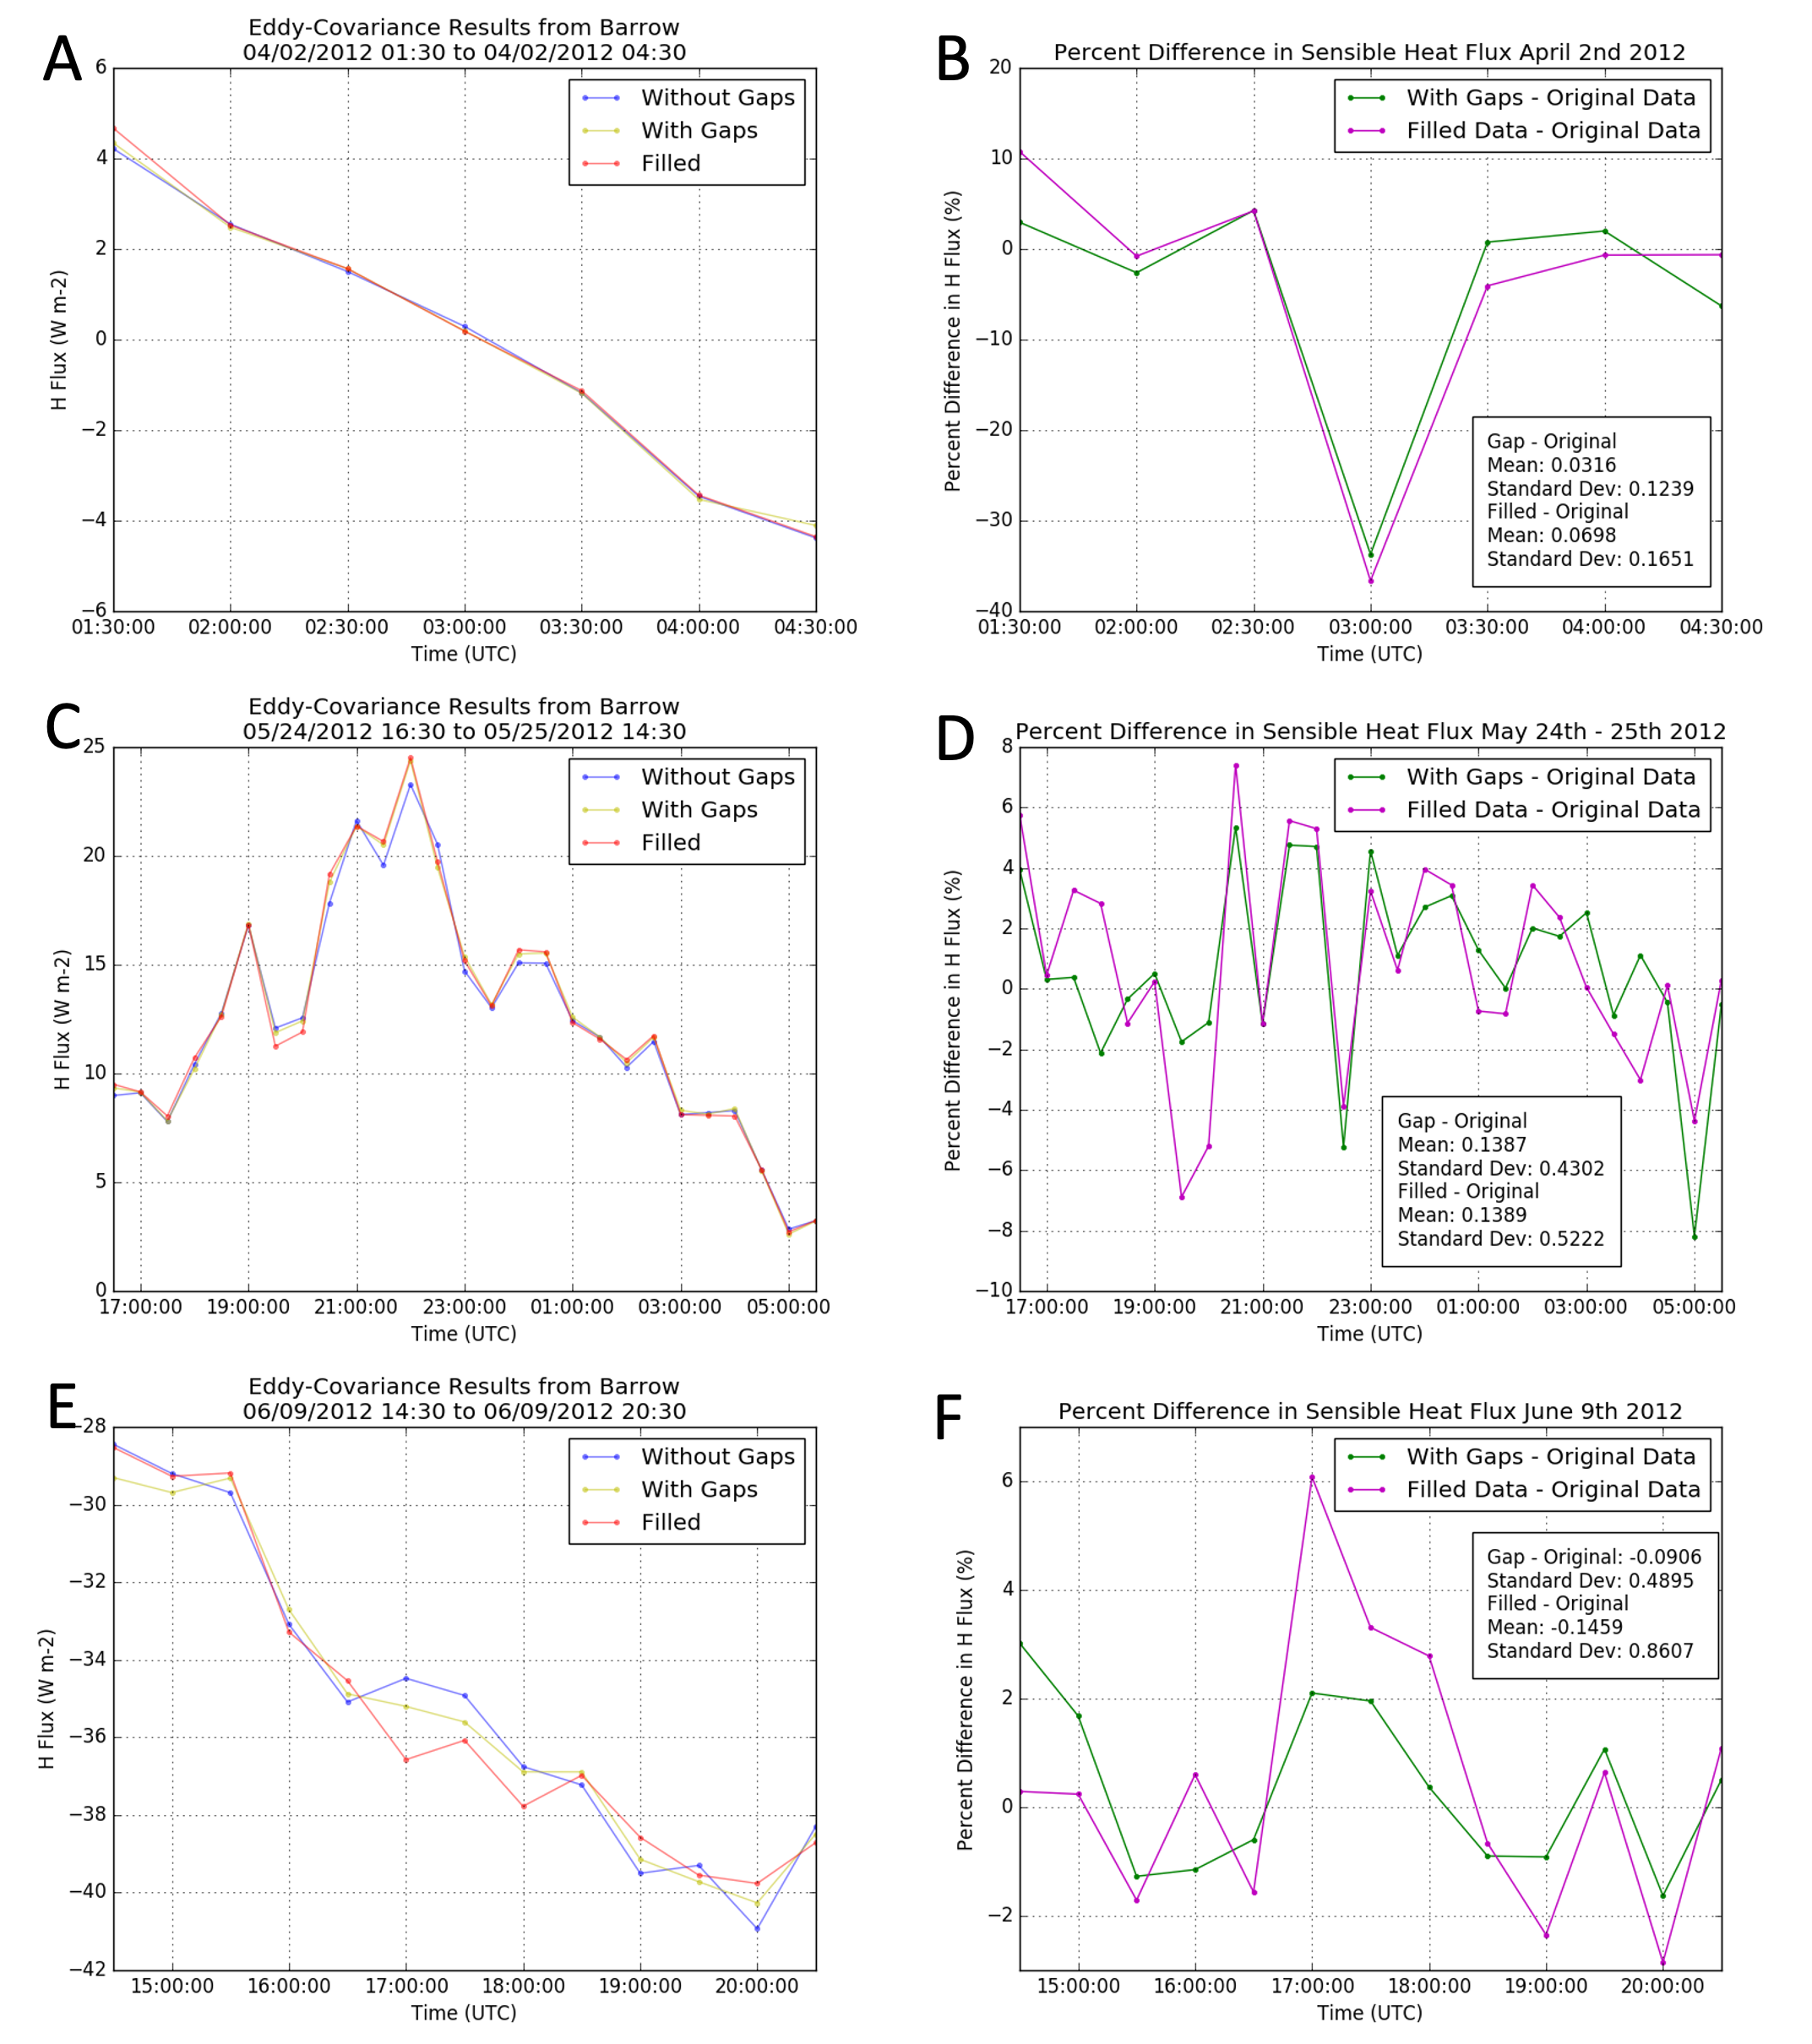
\includegraphics[width=1\linewidth]{figures/appendixb/barrow_fluxes.png}
    \caption[Barrow, Alaska sensible heat flux]{Sensible heat fluxes calculated from the Barrow, Alaska data (left) for April, May, and June. The calculations using the entire dataset (without any artificial gaps) are represented by the blue lines, the calculations done with the data the gaps inserted, but not filled, are shown with the yellow line, and the calculations done with the filled data are shown with the red line. Percent differences from the original, complete dataset are shown on the left. Percent differences calculated using Eq. \ref{eq:withgaps} are shown in green, and Eq. \ref{eq:withoutgaps} are shown in purple. Mean differences and standard deviations are shown for the values (not the percent differences) for both cases in the left figures.}
    \label{fig:barrow_flux}
\end{figure}

The section of data from June again showed that the data with gaps inserted into it did a better job at calculating the fluxes than the data with gaps inserted into it. This section of data contained 13 30-minute data files. The mean difference from the original for the data with gaps was -0.09065 $Wm^{-2}$, and the mean difference from the original for the filled data was -0.14593 $Wm^{-2}$. The sensible heat flux pattern here was captured fairly well by the filled data and the data with gaps, but it can be seen by looking at Figure \ref{fig:barrow_flux} E that the sensible heat flux calculated using the data with gaps did follow the original sensible heat flux pattern better than the filled data calculations did. This is further emphasized in the percent difference figure (Figure \ref{fig:barrow_flux} F), showing that the largest percent difference in sensible heat flux using the data with gaps from the original sensible heat flux was approximately 3 $\%$, while the percent difference using the filled data was as large as 6 $\%$. These percentages are, again, smaller than other months because of the larger magnitude of the sensible heat values, as looking at the time series of sensible heat calculations, a larger discrepancy than in any of the other months can be seen around 1700, yet the percent differences are still smaller than other months.

In each individual month, the data with the gaps inserted into it appeared to portray the original data better than the filled data did when run through EddyPro to calculate sensible heat fluxes. However, all differences were quite small, as could be seen in the mean difference calculations, and the sensible heat flux pattern was conserved throughout calculations using all datasets. Because each dataset from Barrow was relatively small, with the largest dataset containing only 28 points (May), a mean of all Barrow differences was calculated. These means were 0.0593 $Wm^{-2}$, and 0.0498 $Wm^{-2}$ for the filled data calculations and the calculations using the data with gaps, respectively. While this shows that the data with the gaps did a better job at calculating sensible heat fluxes, the differences in these means are so small that it can be said that they both did an acceptable job of estimating sensible heat fluxes. 

It seems intuitive that, because the data with gaps did a better job of calculating the actual sensible heat flux than the filled data did, the data with gaps is a better representation of the heat fluxes. While this may be the case, the filled data was still selected to be used with the N-ICE data. As mentioned in the previous section, EddyPro has a missing data allowance threshold, causing some of the data with a large number of gaps to be removed from processing. Filling the gaps ensures that the data will be processed by EddyPro, making all collected data useable regardless of the gaps. This makes the process of gap filling worth doing, even if it has a slightly larger departure from the actual heat fluxes than the data before the gaps are filled. 

 \subsubsection{Spectral differences}
One of the products calculated by EddyPro is the power spectra of the wind components at a number of frequencies. This shows the frequencies at which the turbulent motion is occurring, higher power indicates that the eddies have more efficient heat transport. Larger eddies have lower frequencies, but often have a greater amount of heat transport as they likely have more mass and momentum. On the other hand, smaller eddies have higher frequencies, and, while they do not have the ability to transport as much heat as a larger eddy, they occur much more frequently \citep{cohen:2015}. 

To determine if we are impacting the power going to the different turbulent spectral frequencies by filling the data, the spectra calculations done with the Barrow dataset were examined. To find the difference between the spectral power at each frequency before and after the filling, the mean monthly percent difference was calculated and is shown in Figure \ref{fig:barrow_diff}. These are not truly monthly means, as they are only a few days of the month at most. It should also be noted that the frequency of the data gaps was determined by the “worst-case scenario” of data gaps in the original dataset. It is likely that larger spectra differences were seen with this situation at specific frequencies due to the regularity of the data gaps and filling. 
Many missing data points existed at high frequencies, so the first 8 frequencies were removed. High-frequency eddies were not impacted by the data-filling method, as can be seen in all plots shown in Figure \ref{fig:barrow_diff}. The largest total impact on the turbulent spectra is seen just after a frequency of 10-2 Hz. At this point, spikes in the turbulent spectra of all components of the wind ($W$, $V$, and $U$) can be observed. The largest spikes at this point are the $V$ wind component spectra, reaching as high as approximately 450 $\%$ difference in April. A second spike can be seen just after the first, halfway between 10-2 and 10-1 $Hz$. The $V$ component of the wind is, again, the most impacted at this frequency for almost all of the months. An exception is in May, where the $U$ component of the wind has a slightly larger percent difference than the $V$ component. These two frequencies are the only frequencies at which percent differences exceed 100 $\%$ of the original. This indicates that the frequencies affected most by the data filling are at approximately 0.0192 $Hz$ and 0.2257 $Hz$. It is important to be aware that turbulent energy at these frequencies is affected by the gap-filling process.

  \begin{figure}[h]
    \centering
    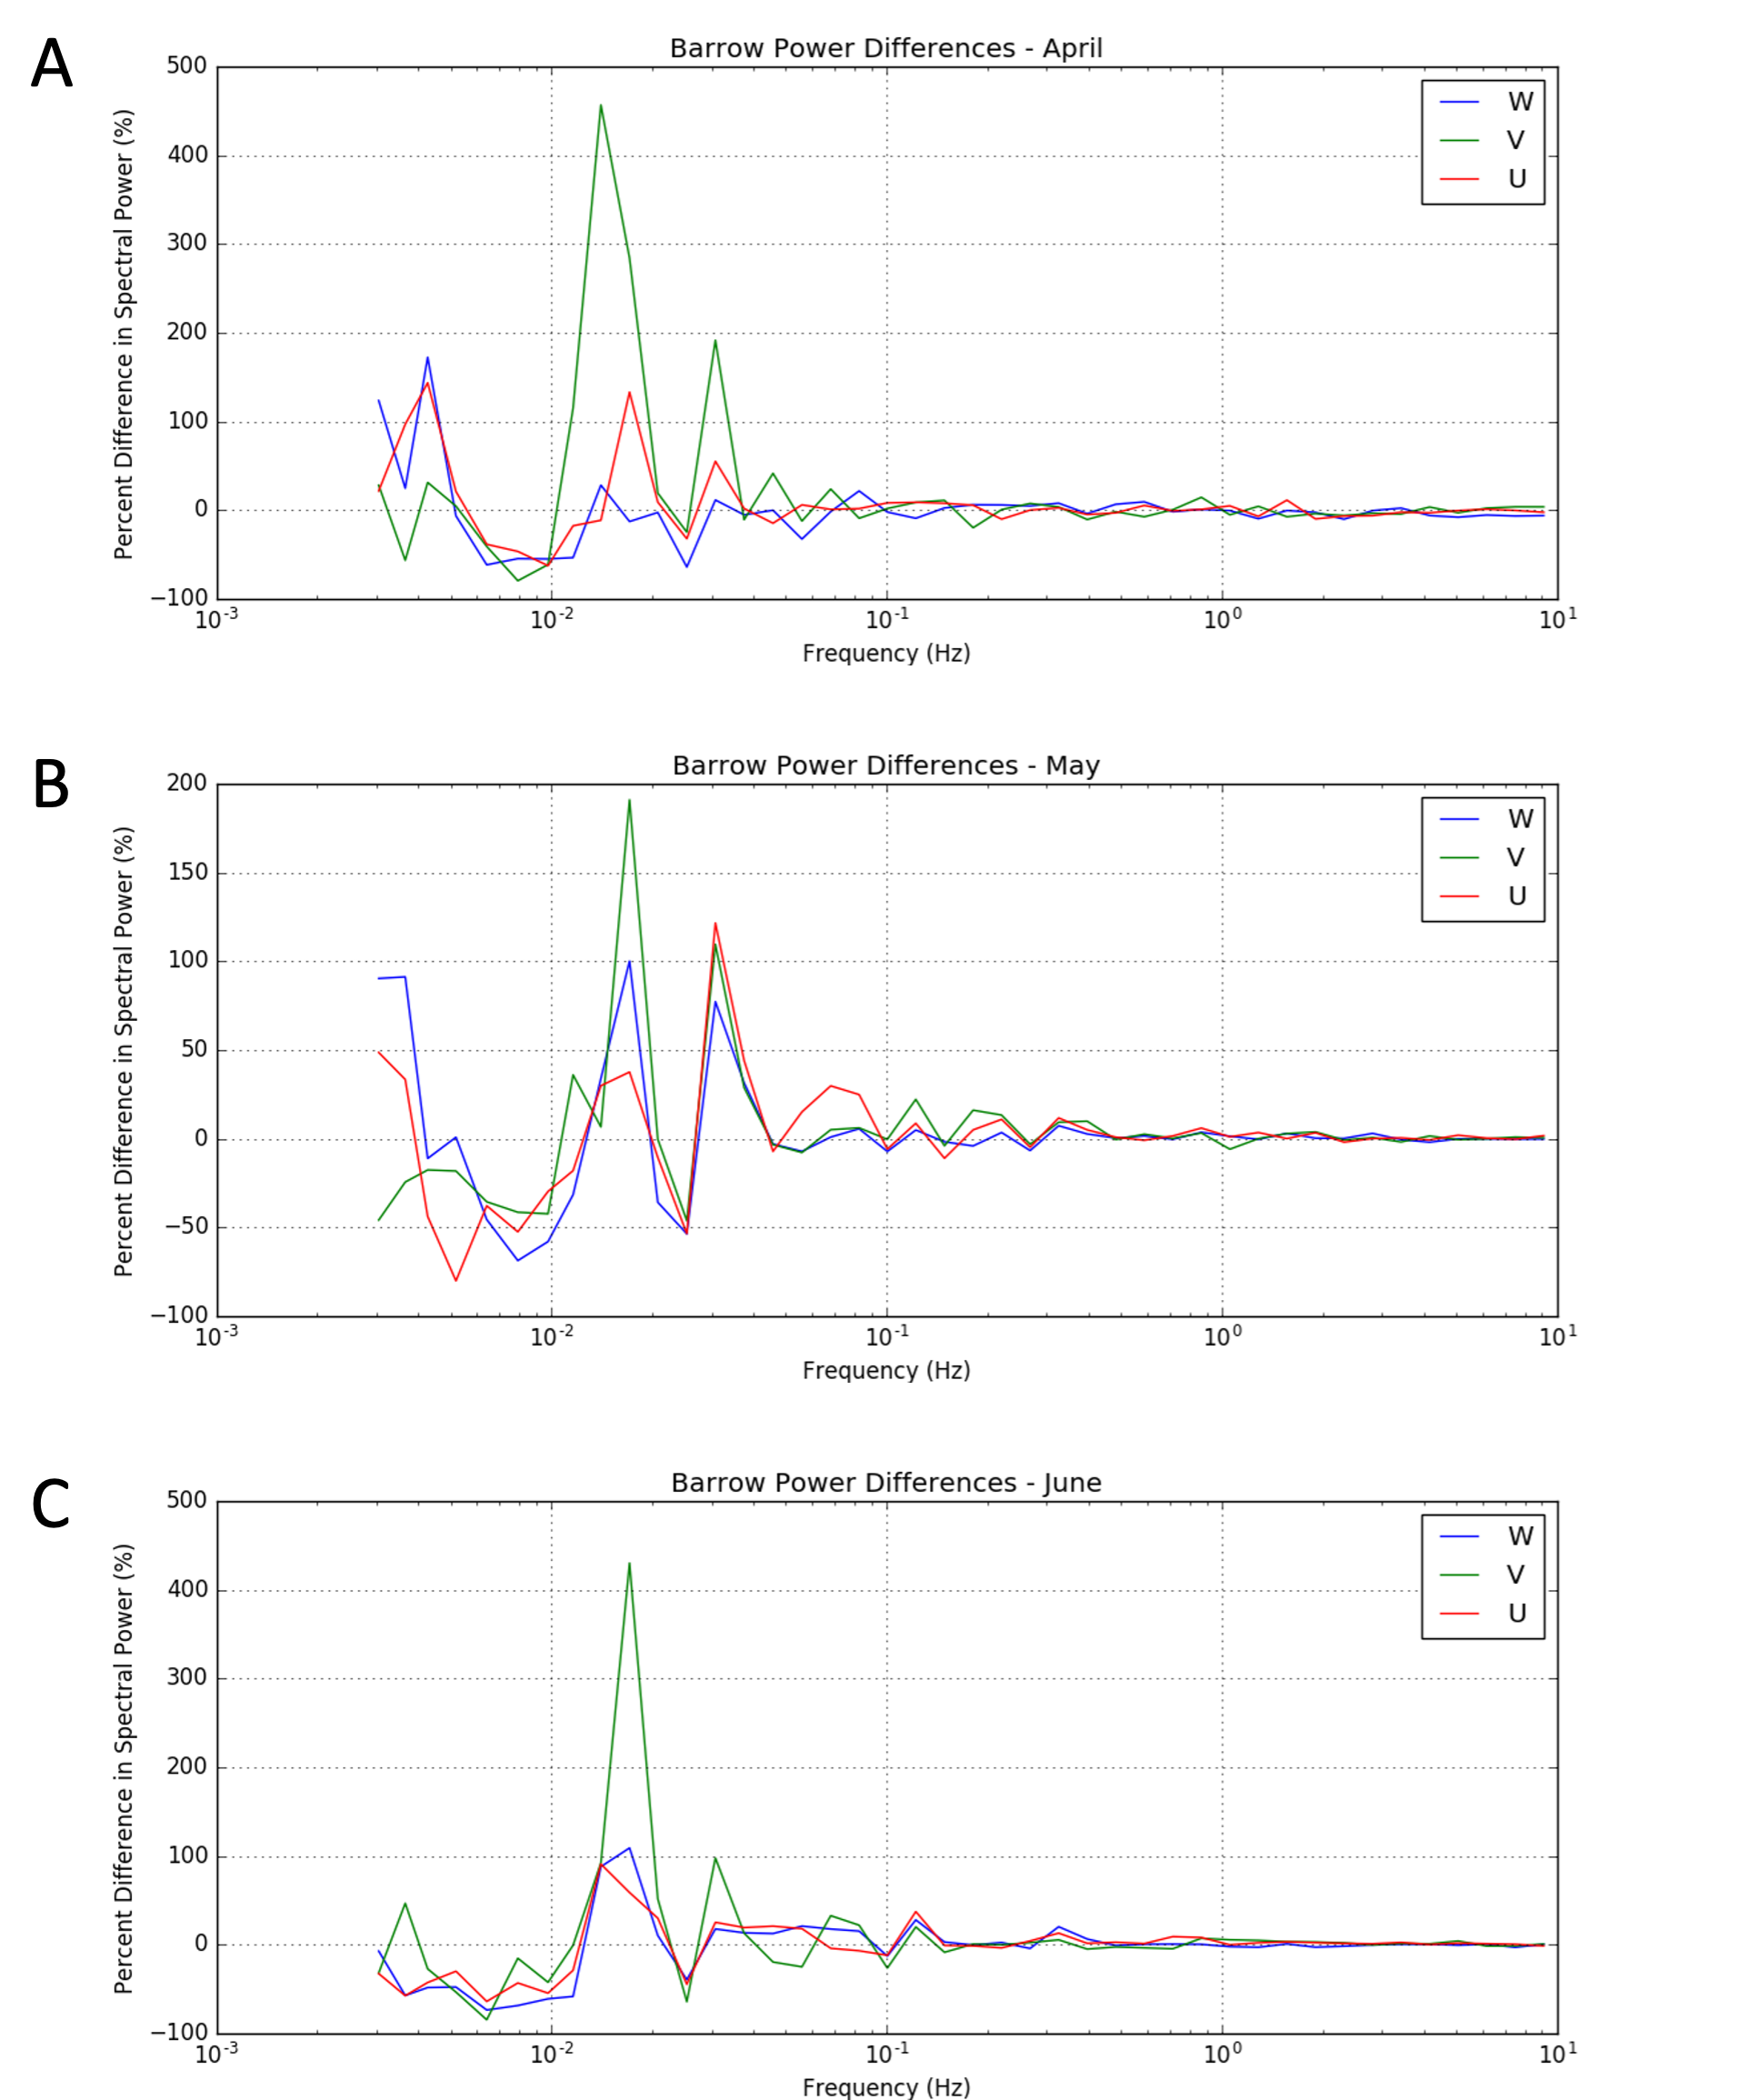
\includegraphics[width=1\linewidth]{figures/appendixb/barrow_power_april.png}
    \caption[Barrow, Alaska power spectra]{The percent difference in mean monthly spectra calculated by the filled data from the original data (Eq. \ref{eq:withgaps}) for April, May, and June. The W, V, and U components of the wind are shown in blue, green, and red, respectively.}
    \label{fig:barrow_diff}
\end{figure}


\subsection{N-ICE Filled Data Comparison}

When comparing the time series of filled data with the data containing gaps from the N-ICE project, there is not an obvious difference in the calculated sensible heat fluxes. Examining the time series for section 1 (Figure \ref{fig:nice_fluxes} A) shows little to no difference between the two. Figure \ref{fig:percent_diff} A displays the percent differences between the two calculations and shows that the differences are close to zero until the last day of the dataset, with the largest difference not exceeding 200 $\%$ of the heat flux calculation by the original dataset. In addition, this difference occurs during an apparent data spike, which is likely not an accurate measurement. Regardless of the spike, this difference is relatively low compared to the differences found in the other two sections (Figure \ref{fig:nice_fluxes} B and Figure \ref{fig:nice_fluxes} C and Figure \ref{fig:nice_fluxes} B and Figure \ref{fig:nice_fluxes} C), where magnitudes of differences can reach as high as over 2000 $\%$. It should be noted that in section 3 there is a location with a difference of 30 $Wm^{-2}$, which equates to over a 10000 $\%$ difference (around 25 May), but this is just one point, and when compared with the time series shown in Figure \ref{fig:barrow_diff}, it becomes obvious that this is the location of a spike that is likely an error in the data, and not necessarily a calculation error. The largest differences often occur when these spikes occur, indicating something else interfering with the data other than the filling calculations. When these spikes are disregarded, percent differences generally stay around or under 500 $\%$, with some exceptions in the second and third sections of data. Throughout the entire time series shown in Figure \ref{fig:nice_fluxes}, the patterns seen in the sensible heat flux are conserved in both calculations. This further confirms that the filling of the data, while often making the flux calculations a bit further from the actual fluxes, can conserve any trends in the data while ensuring that all files can be used in the calculation. 

 \section{Future Work}
The best option for improving any data-filling method is eliminating the need for it. An examination of the instruments used for this project along with any external factors that could be influencing the data collection should be conducted to determine why these semi-regular and random data gaps are occurring throughout the data set. While some gaps in data can be expected, something had to have been causing the semi-regular data gaps to occur for one minute every five minutes throughout the majority of the project. At this point, however, determining the source of error in the instruments will not help this dataset, but could improve data collection in the future, removing the need for a data-filling method.
The next steps in this project are expanding the dataset the method is being checked with or using a different dataset with more similar conditions to the N-ICE data. The dataset from Barrow, Alaska used, while complete, was a tiny dataset, and was not over newly formed sea ice. Using a longer dataset would improve the percent differences in the turbulent spectra, as these were averages over the short period of time used here. 

  \begin{figure}[h]
    \centering
    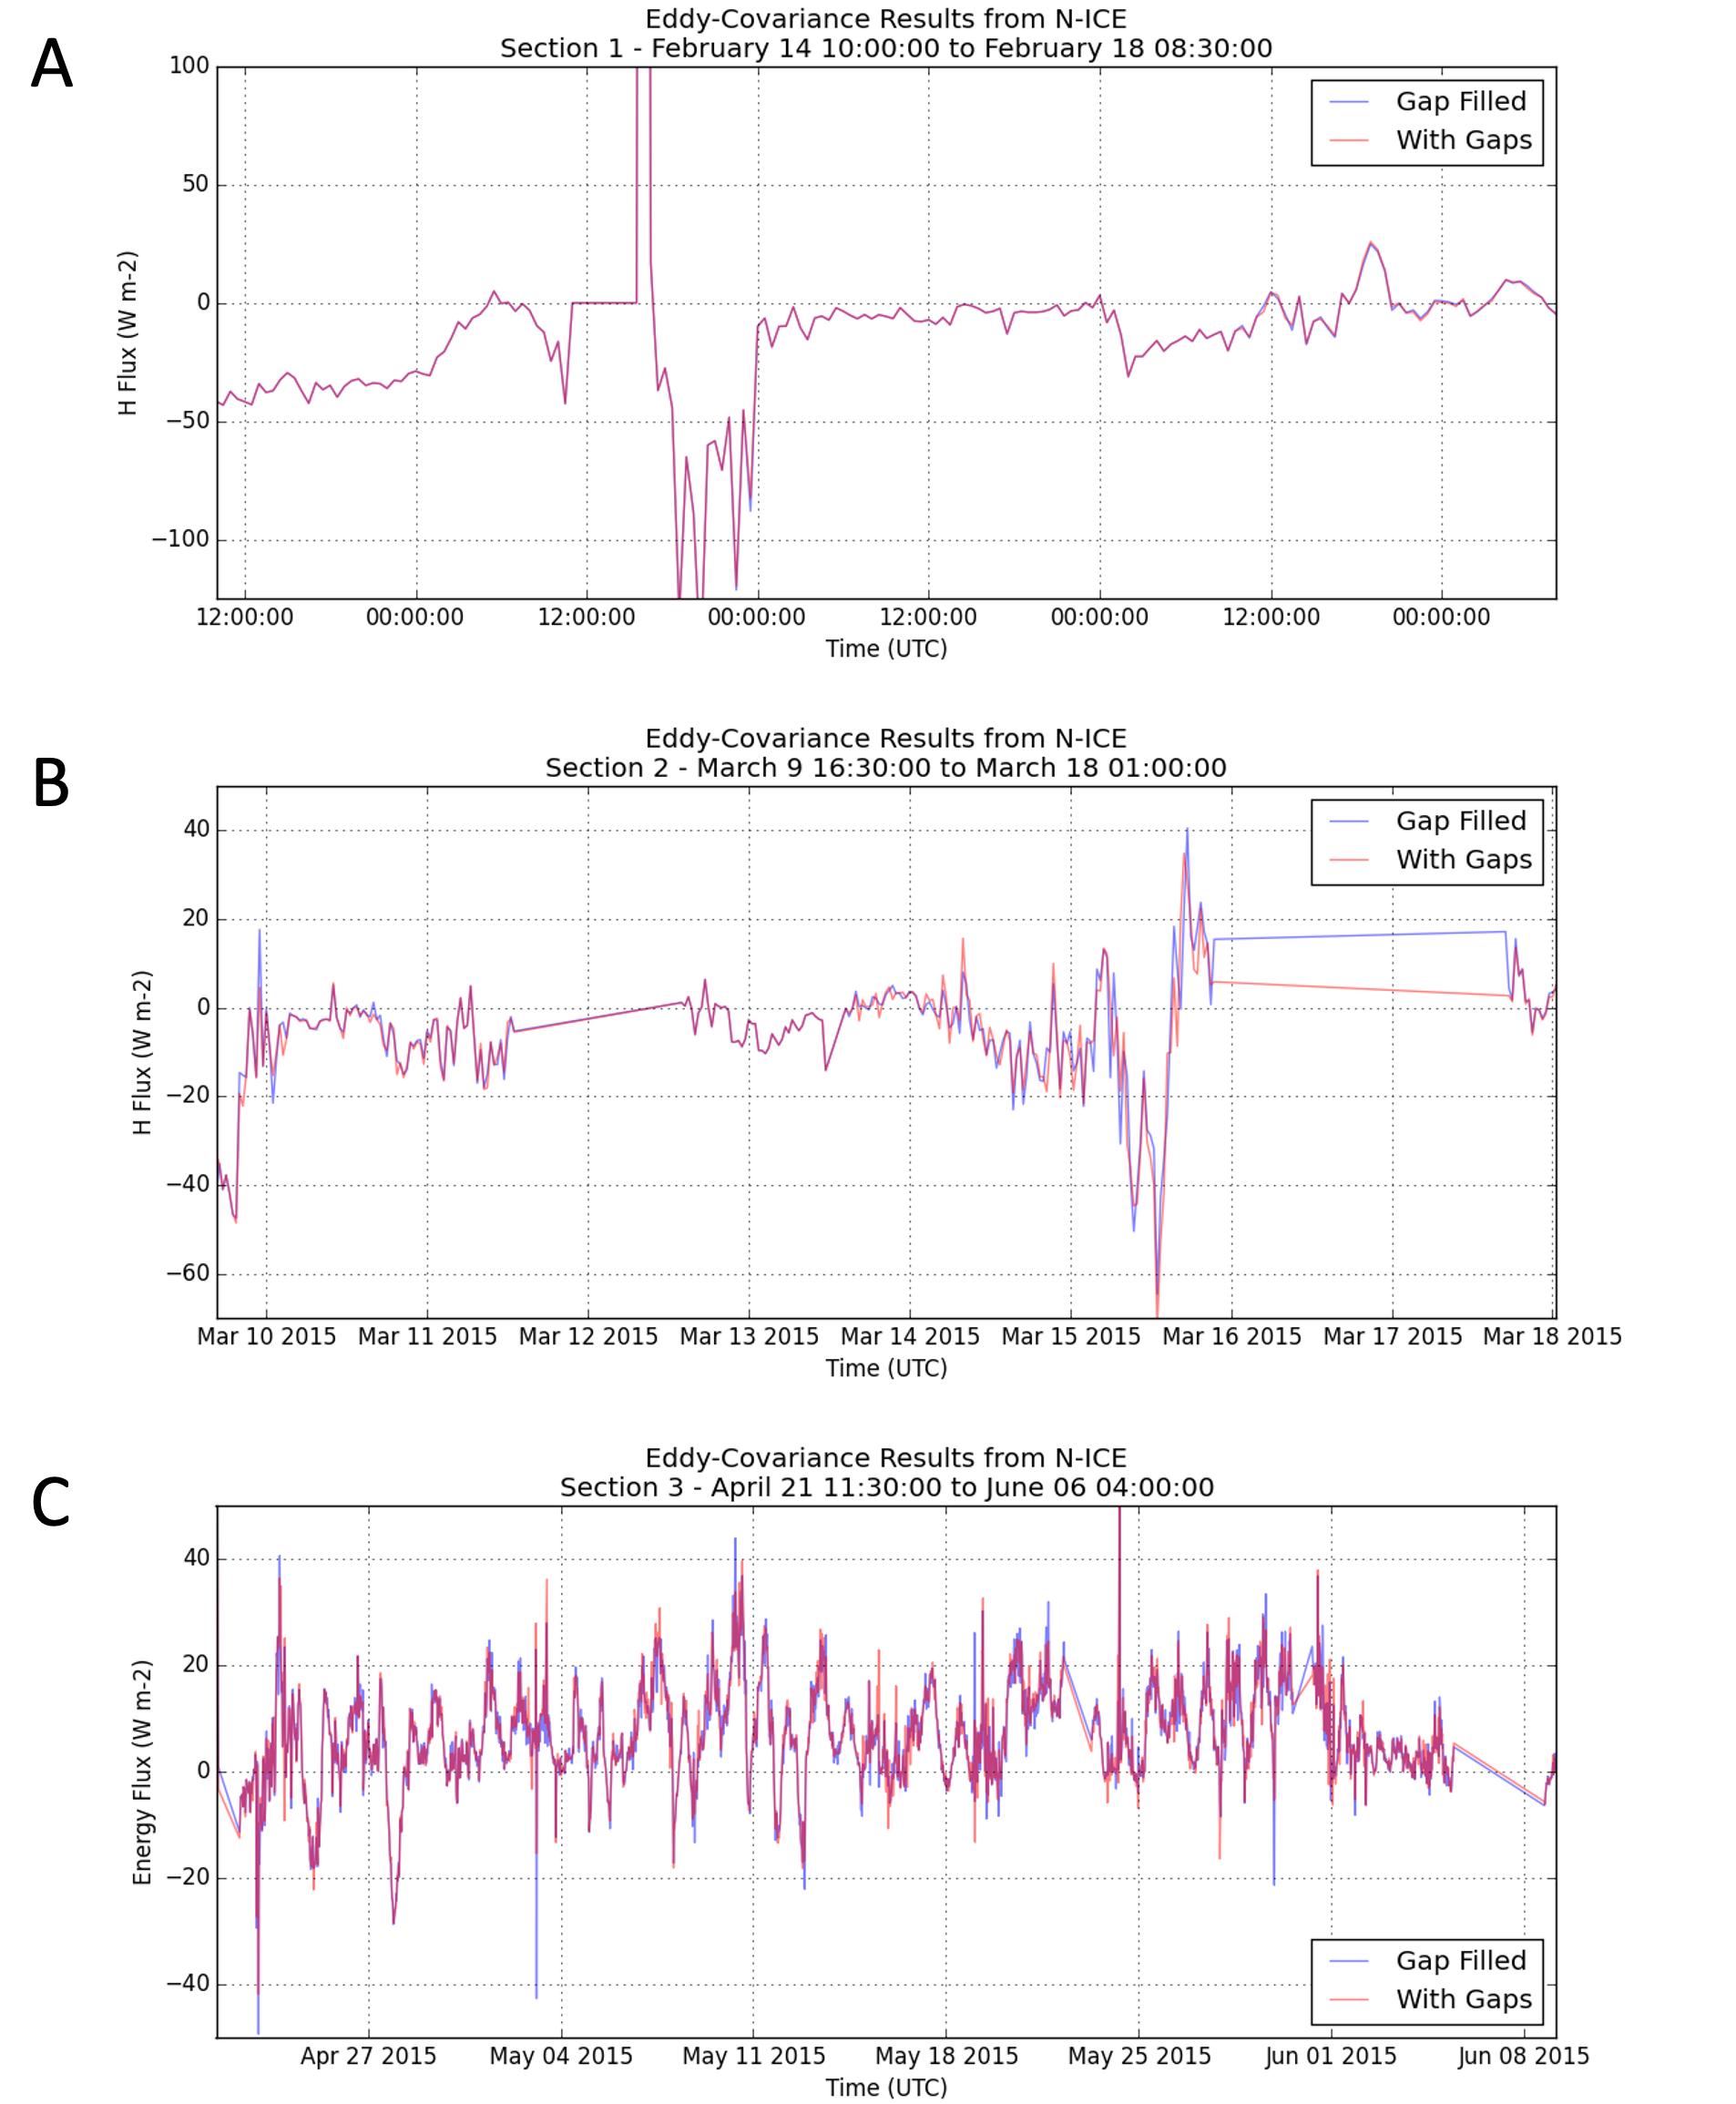
\includegraphics[width=1\linewidth]{figures/appendixb/nice_fluxes.png}
    \caption[N-ICE sensible heat flux]{Sensible heat flux ($Wm^{-2}$) values for each of the three sections of N-ICE data. Both calculations were done with the original data (with gaps, shown in red), and the filled data (gap filled, shown in blue).}
    \label{fig:nice_fluxes}
\end{figure}

  \begin{figure}[h]
    \centering
    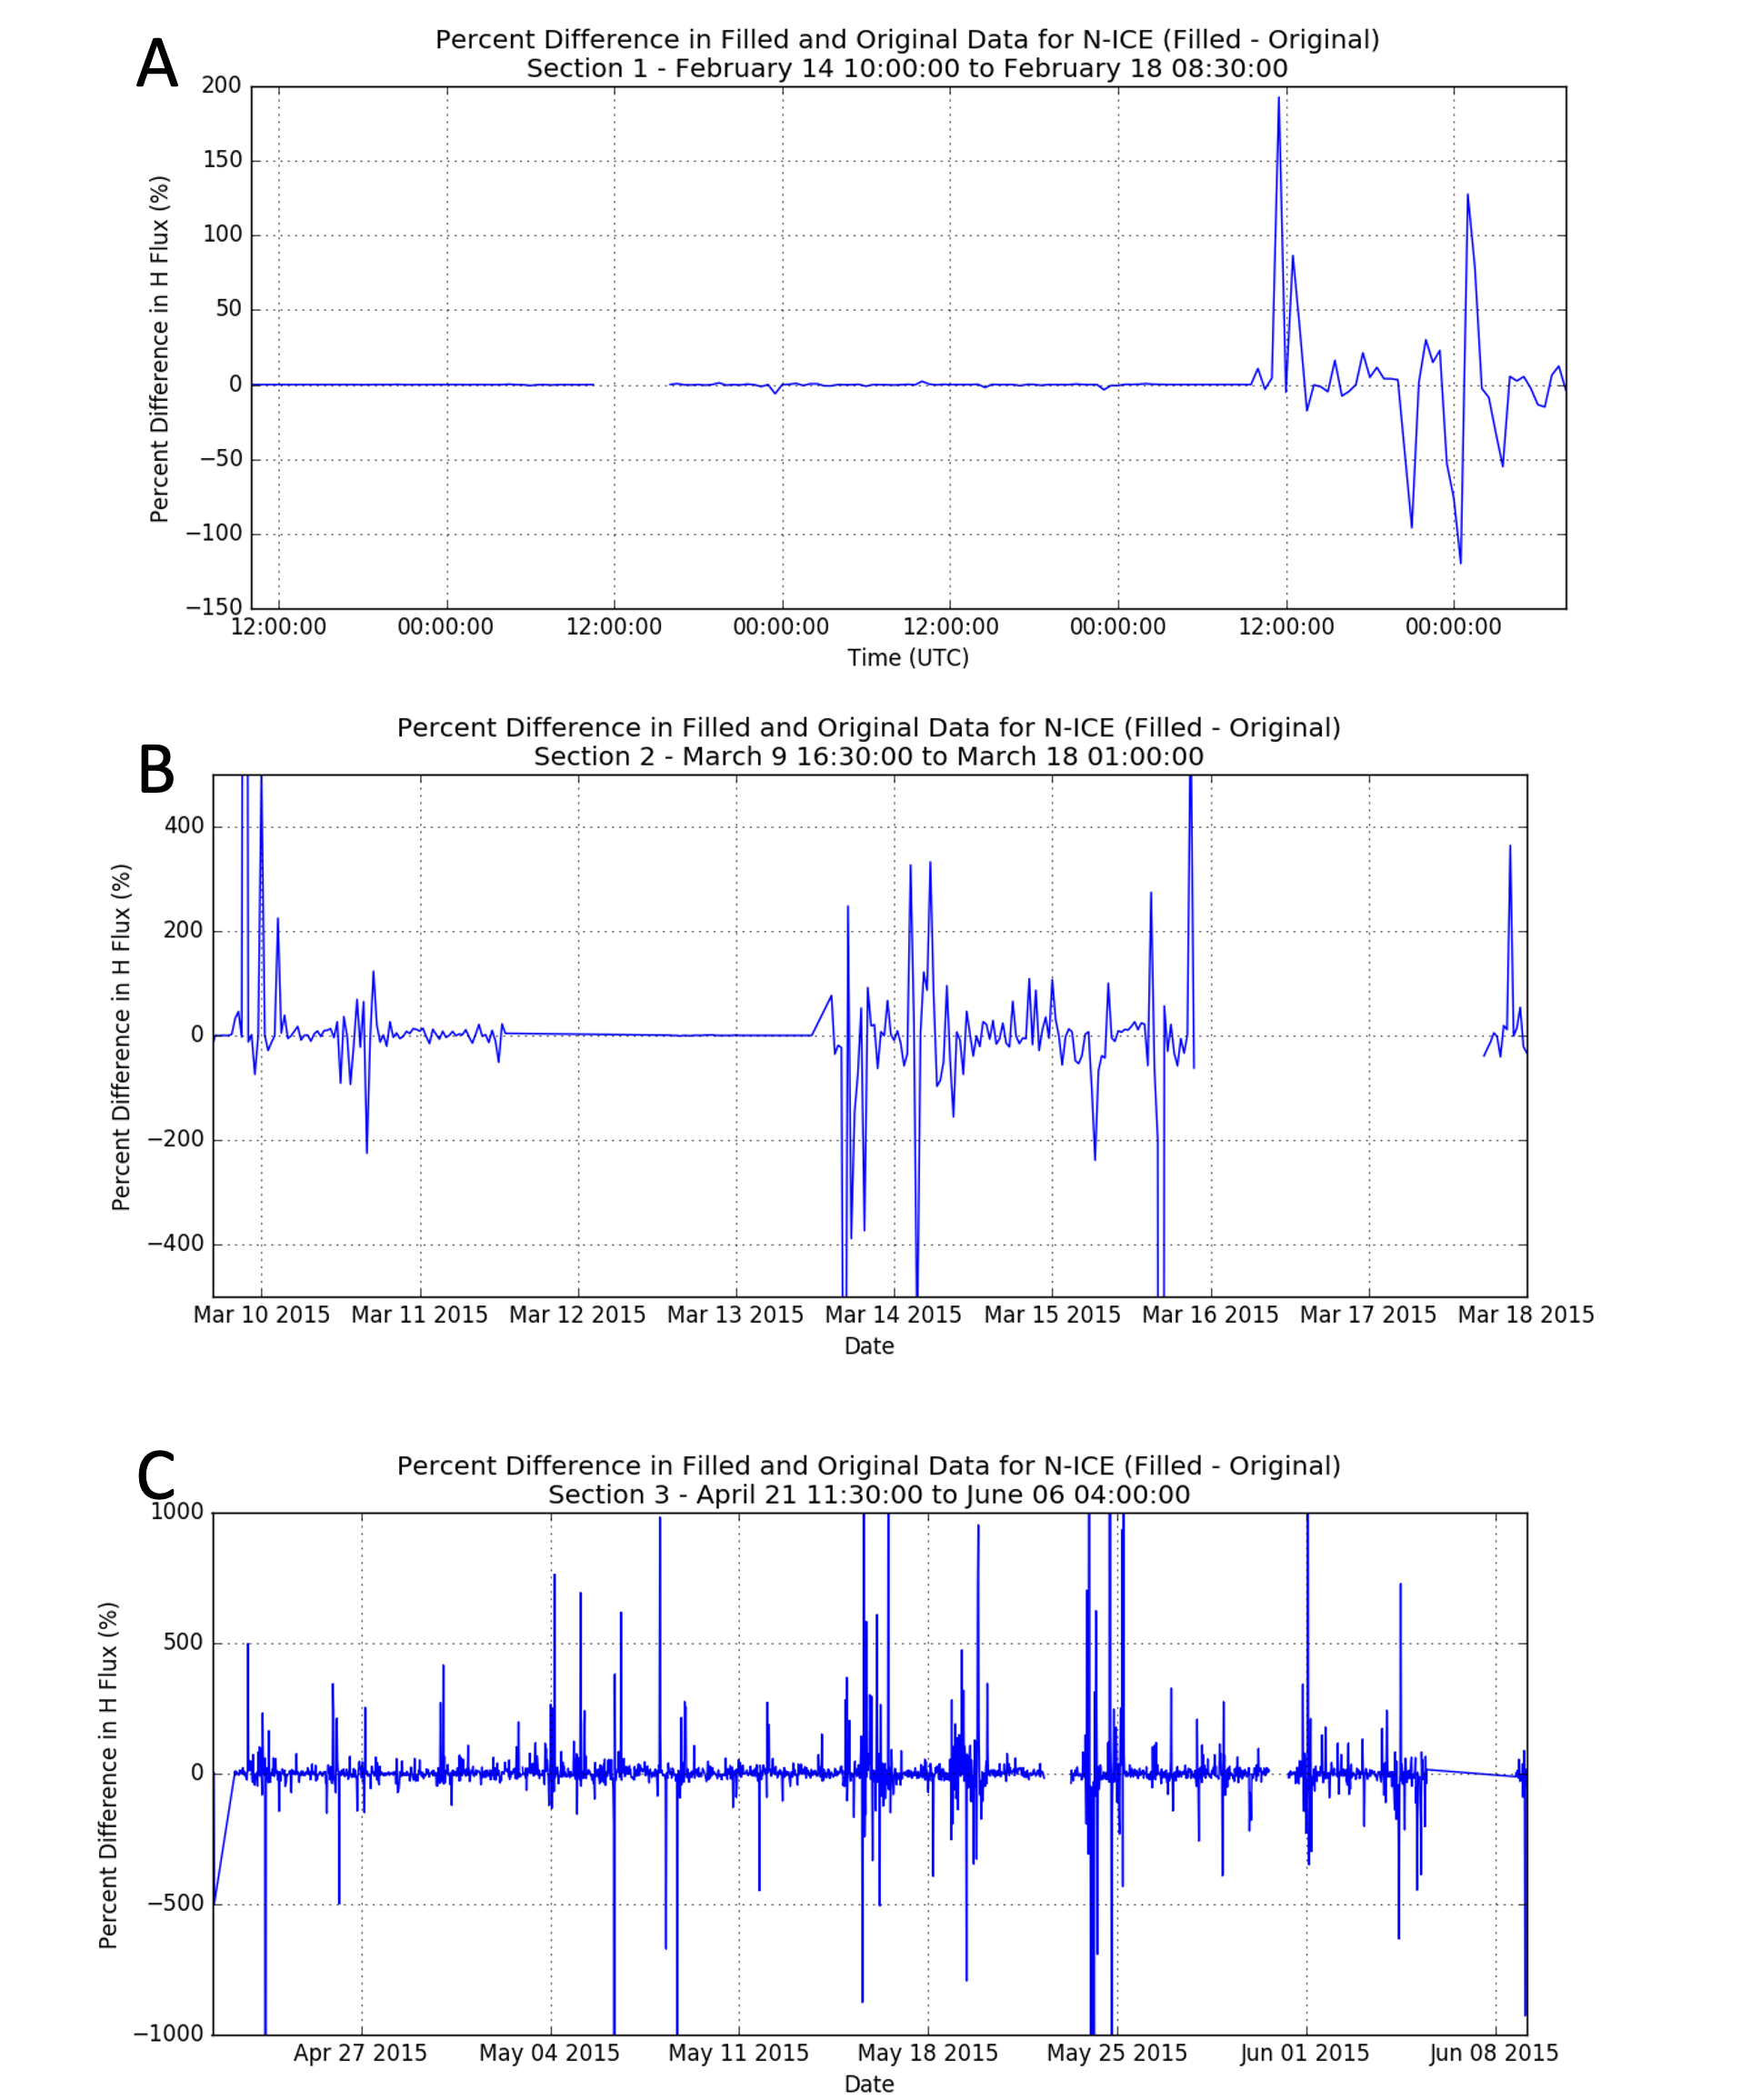
\includegraphics[width=1\linewidth]{figures/appendixb/percent_diff.png}
    \caption[N-ICE percent differences between filled and unfilled datasets.]{The percent differences between the original dataset and the filled N-ICE dataset (each dataset shown in Figure \ref{fig:nice_fluxes}). Percent differences were calculated by subtracting the filled calculations from the original (data with gaps) and dividing by the original values, then multiplying by 100. Note the differences in axis range from one section to the next.}
    \label{fig:percent_diff}
\end{figure}

Another thing to consider when studying the results presented here is the meteorological conditions occurring. If meteorological data were compared to the differences in the fluxes calculated by the original and filled data from Barrow, it is possible that it could be determined what conditions this filling works best in and where it is less effective. This could help to determine if this data-filling method is the correct one for certain project sites. In addition, looking at the changes in the latent heat flux could also give valuable information about how the data filling is impacting the data processing. Lastly, inserting a variety of different gaps into the test dataset would give valuable information about the size of the gaps that this filling technique is effective for and how random data gaps change the turbulent spectra. 

 \section{Conclusion}
The N-ICE dataset has a number of problems, including sections of missing data. Some of the data is missing at regular intervals and some sections of missing data are random. Because of the missing data allowance threshold that EddyPro holds the data to, some of the 30-minute data files were being removed from processing, leading to an (even more) incomplete set of data. To fix this problem, a filling technique needed to be developed that did not negatively impact the calculations of the sensible heat flux.

The technique of filling gaps in eddy covariance data with a replica of the section of time before (or after, if there is not enough data before the gap) is shown to conserve trends in sensible heat flux data after processing. Small percent differences between known sensible heat flux values and sensible heat flux values calculated with the filled data were seen (less than 10 $\%$ with the exception of one point) when the filling technique described here was applied to a complete dataset with artificial data gaps inserted into it. In addition, spectral power showed small differences for most frequencies with the exception of two, showing the frequencies at which the gap filling influences the spectra, and indicating that the filling does have an impact on the calculated turbulent spectra. This filling technique was deemed acceptable for use with the N-ICE data after examination of the Barrow, Alaska results. This data filling results in a higher number of files being accepted into EddyPro.

